%/*******************************************************************************
% * Copyright (c) 2009, medshare GmbH
% * All rights reserved. This program may not be distributed
% * or modified without prior written consent
% *
% * Contributors:
% *    T. Schaller - initial implementation
% *
% *******************************************************************************/
\documentclass[a4paper]{scrartcl}
\usepackage{german}
\usepackage[utf8]{inputenc}
\usepackage{makeidx}
\usepackage{wrapfig}
\makeindex

\usepackage[pdftex]{graphicx}
\DeclareGraphicsExtensions{.pdf,.jpg,.png}

\usepackage{floatflt}
\usepackage[]{hyperref}
\usepackage{color}
\title{Elexis - Reflotron Connector}
\author{medshare GmbH}

\def\<{{\tt\char'74}}
\def\>{{\tt\char'76}}

\begin{document}

\maketitle
	\begin{center}
		
\includegraphics{elexis_logo}
	\end{center}
	\begin{center}
		
\includegraphics{roche_logo}
	\end{center}
	\begin{center}
		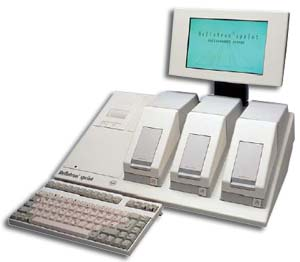
\includegraphics{reflotron_device}
	\end{center}
\pagebreak


\section{Einf\"uhrung}
Dieses Plugin dient dazu, die Laborger\"at 'Reflotron sprint' und 'Reflotron plus' \footnote{Firma Roche Diagnostics} an Elexis anzubinden. Mit diesem Plugin k\"onnen die, vom Reflotron gemessenen Laborparameter direkt in die Elexis-Datenbank eingelesen werden.

\subsection{Voraussetzungen}
Dieses Plugin ben\"otigt Elexis V1.4.1 oder h\"oher sowie einen Reflotron Ger\"at (Modell sprint oder plus). Ausserdem wird ein PC mit mindestens einer freien seriellen Schnittstelle und ein korrekt gerade verdrahtetes serielles Kabel (kein Nullmodemkabel) zur Verbindung des Reflotrons mit dem PC ben\"otigt \footnote{Alternative: RS-232 Adapter f\"ur USB oder Bluetooth}.

\section{Installation und Konfiguration}
Installieren Sie auf dem, sich im Labor befindlichen PC das Plugin wie gewohnt. Verbinden Sie dann bei \textbf{ausgeschalteten} Ger\"aten den Reflotron mit einem seriellen Port des Computers. 
\subsection{Daten\"ubertragung am Reflotron einschalten}
Die serielle Datenkommunikation ist im Reflotron standardm\"assig inaktiv. Damit das Reflotron Ger\"at Daten \"uber die Schnittstelle an den Computer sendet, muss die Daten\"ubertragung eingeschaltet werden. Wie dies gemacht wird, ist im Manual zum Reflotron im Kapitel 6 (Insbesondere Seite 6.9) beschrieben. Es folgt hier nur eine Kurzform f\"ur ge\"ubte Techniker:\\
\\
\textbf{Reflotron sprint:}\\
F2, User Level Setup\\
Fn+F1 (=F11)\\
Lowlevel Passwort: LOW LEVEL\\
2x Pg Down\\
RS-232\\
Mit Esc zur\"uck bis zur Hauptmaske (Werte sind gespeichert).\\
\\
\textbf{Reflotron plus:}\\
Ger\"at ausschalten\\
Tasten \< und \> gleichzeitig dr\"ucken und Ger\"at einschalten\\
Erste 10 Eintr\"age mit Enter best\"atigen; bis Baudrate erscheint\\
Einstellungen (siehe unten) falls notwendig mittels Tasten \< und \> ver\"andern\\
Weitere 5 Eintr\"age mit Enter best\"atigen; bis 'SETUP OK ?' erscheint\\
\\
\\
\textbf{Roche empfiehlt folgende Einstellungen:}\\
Baudrate: 9600\\
Stop-Bits: 1\\
Parity: None\\
STX/ETX Frame: Yes\\
Automatic Data Transfer To RS 232: Yes\\
BCC: Odd (kann in Elexis nicht eingestellt werden)\\

\subsection{Elexis Konfiguration}
Starten Sie Elexis und gehen Sie dort zu \textsc{Datei-Einstellungen-Datenaustausch-Roche Reflotron} (S. Abb. \ref{fig:config}).
\begin{figure}[h]
    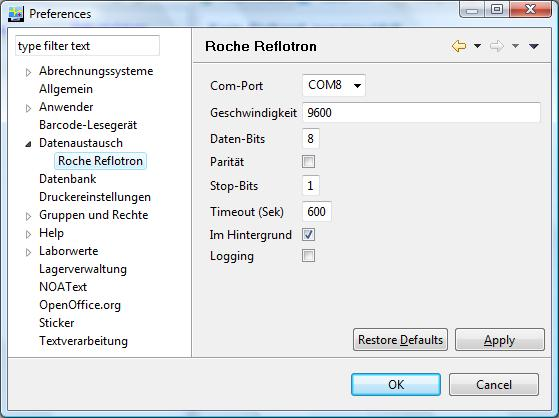
\includegraphics{config}
    \caption{Einstellungen Reflotron}
    \label{fig:config}
\end{figure}
Hier stellen Sie den seriellen Port und die Schnittstellenparameter ein. Die Werte m\"ussen mit den Einstellungen auf dem Reflotron Ger\"at \"ubereinstimmen (siehe oben). Wichtig: Nach dem \"Andern dieser Parameter m\"ussen Sie Elexis neu starten.\\
\\
\textbf{Weitere Konfigurationswerte:}\\
\textbf{Timeout (Sek):} Der Wert bestimmt, wie lange Elexis maximal auf Resultate warten soll, bevor die Verbindung getrennt wird.\\
\textbf{Im Hintergrund:} Damit beeinflussen Sie das Verhalten von Elexis. Bei eingeschalteter Option wird die \"Ubertragung im Hintergrund ausgef\"uhrt und Sie k\"onnen weiter in Elexis arbeiten. Bei ausgeschalteter Option erscheint die Abb. \ref{fig:connected}\\
\textbf{Logging:} Diese Option verwenden Sie bitte nur auf Anweisung des Supports, ansonsten wird Ihr Computer mit unn\"otigen Daten gef\"ullt.\\
\section{Verwendung}
Wenn das Plugin korrekt installiert ist, erscheint in der Labor-View automatisch ein neuer Toolbar Button 'Reflotron' (Abb. \ref{fig:toolbarbutton}). Klicken Sie auf diesen Knopf um die Verbindung mit dem Ger\"at herzustellen. 
\begin{figure}[h]
    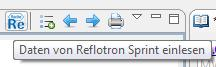
\includegraphics{toolbarbutton}
    \caption{Reflotron Daten einlesen}
    \label{fig:toolbarbutton}
\end{figure}
Die Verbindung bleibt bestehen bis das Timeout gem\"ass Konfiguration abgelaufen ist. Das Reflotron Ger\"at ben\"otigt f\"ur die verschiedene Tests unterschiedlich lang. Jedesmal wenn ein Test abgeschlossen ist, wird das Resultat an den Computer gesendet. Wenn alle Resultate empfangen wurden, kann die Verbindung abgebrochen werden (Cancel gem\"ass Abb. \ref{fig:connected}).
\begin{figure}[h]
    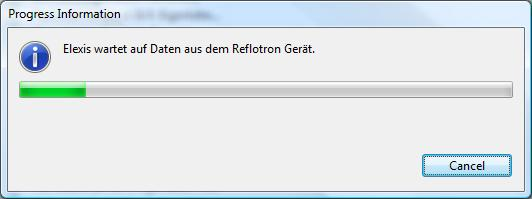
\includegraphics{connected}
    \caption{Verbindung zum Reflotron ist aufgebaut}
    \label{fig:connected}
\end{figure}
\begin{figure}[h]
    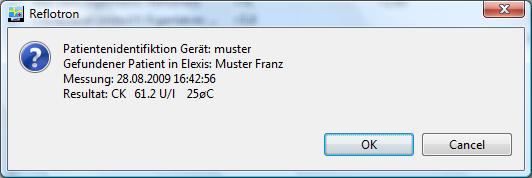
\includegraphics{messwert}
    \caption{Messwert vom Reflotron eingetroffen}
    \label{fig:messwert}
\end{figure}
Wenn Elexis ein Resultat empf\"angt, wird versucht, dieses einem Patienten zuzuordnen. In Abb. \ref{fig:messwert} ist ersichtlich, wie der Patient zugeordnet wird (Beispiel: Muster Franz sind die Angaben aus Elexis und muster wurde auf dem Reflotron eingegeben). Kann der Patient nicht automatisch zugewiesen werden folgt das Fenster mit der Patientenselektion.\\
\\
Es kann passieren, dass der Datenstrom zwischen Reflotron und Computer fehlerhaft ist. In diesem Fall erscheint eine Fehlermeldung (siehe \ref{fig:transmissionerror}). In diesem Fall kann das Profil des Patienten auf dem Reflotron erneut gesendet werden.\\
\begin{figure}[h]
    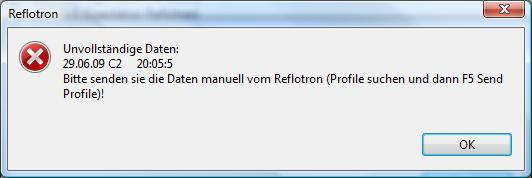
\includegraphics{transmissionerror}
    \caption{Fehlerhafte Daten vom Reflotron eingetroffen}
    \label{fig:transmissionerror}
\end{figure}
\\
\textbf{Reflotron sprint:}\\
F2, Profil aufrufen, F10 Patient suchen und F5 Send Profile\\
Eine genauere Anleitung befindet sich im Manual zum Reflotron auf S. 3.21.\\
\\
\textbf{Reflotron plus:}\\
F9, Patientennamen eingeben (achten Sie auf Gross-/Kleinschreibung), Enter\\
Eine genauere Anleitung befindet sich im Manual zum Reflotron auf S. 6.10.\\
\textbf{Wichtig:} Das \"Ubertragungsprotokoll bei Benutzung der Funktionstaste F8 ist nicht unterst\"utzt!\\
\\
\subsection{Anweisungen zum Reflotron}
Damit eine automatische Zuweisung des Patienten m\"oglich wird, muss auf dem Reflotron der Patient der Messung zugeordnet werden. Sie m\"ussen zwingend eines der folgenden Eingabeformat einhalten (ohne Leerzeichen nach dem Komma!):\\
\begin{itemize}
\item \textbf{PatNummer,Namen}\\Tipp: Es kann auch nur der erste Buchstabe des Namens eingegeben werden
\item \textbf{Namen,Vornamen}\\Tipp: Namen und/oder Vornamen k\"onnen auch abgek\"urzt eingegeben werden
\end{itemize}
Den Patientennamen k\"onnen Sie nach Dr\"ucken der Taste Home erfassen und mit Enter auf die aktive Messkammer \"ubernehmen. Das m\"ussen Sie tun, bevor Sie die Messkammer schliessen.\\
\\
Das Reflotron verlangt von Zeit zu Zeit die Checkstreifen. Bei solchen Check Messungen messen Sie keine Patienten Proben in einer andern Messkammer und stellen Elexis dabei auch nicht auf Empfang. Die Fehlermeldung des Ger\"ates 'Kein Datentransfer'  k\"onnen Sie in diesem Fall ignorieren.
\subsection{Hinweise zu Testserien am selben Tag (z.B. Glucose)}
Elexis unterst\"utzt nur ein Messwert pro Patient, Datum und Zeile im Laborblatt. Bei Testserien (z.B. mehrere Glucosetests) m\"ussen Sie deshalb manuelle Eintr\"age im Laborblatt erstellen und im Falle von Testserien jeweils nach der \"Ubermittlung die Einzelresultate diese manuell in die daf\"ur vorgesehenen Zellen \"ubertragen.\\
\textbf{Wichtig:} Beim \"Ubermitteln des n\"achsten Testresultates mit dem selben Datum wird das vorherige Laborresultat in Elexis \"uberschrieben!
\section{Plattformen}
Dieses Plugin wurde unter Windows XP und Vista getestet. Beachten Sie bitte, dass unter Linux die seriellen Ports nicht COM1 usw., sondern /dev/ttyS0 usw. heissen.
\section{Kabelspezifikation}
\begin{figure}[h]
    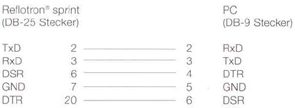
\includegraphics{kabel}
    \caption{Reflotron Kabelkonfiguration}
    \label{fig:kabel}
\end{figure}
Es wird ein normales, serielles Kabel ben\"otigt (kein Nullmodemkabel!). Das Kabel muss vom 25-poligen Stecker (m\"annlich) auf den 9-poligen Stecker (weiblich) gem\"ass Abb. \ref{fig:kabel} verdrahtet sein.
\end{document}
